\documentclass{article} % For LaTeX2e
\usepackage{nips12submit_e,times}
\usepackage{amsmath,bbold}
\usepackage{graphicx}
%\documentstyle[nips12submit_09,times,art10]{article} % For LaTeX 2.09
\newcommand{\tab}{\hspace*{2em}}

\title{Citation Recovery with Weighted Citation Network Links and Contextual Semantic Information}


\author{
Jonathan C. Barker\tab Kartik Goyal\tab Zhengzhong Liu \\
Language Technologies Institute \\
Carnegie Mellon University \\
Pittsburgh, PA 15213 \\
\texttt{\{jcbarker, kartikgo, liu\}@cs.cmu.edu} \\
}

% The \author macro works with any number of authors. There are two commands
% used to separate the names and addresses of multiple authors: \And and \AND.
%
% Using \And between authors leaves it to \LaTeX{} to determine where to break
% the lines. Using \AND forces a linebreak at that point. So, if \LaTeX{}
% puts 3 of 4 authors names on the first line, and the last on the second
% line, try using \AND instead of \And before the third author name.

\newcommand{\fix}{\marginpar{FIX}}
\newcommand{\new}{\marginpar{NEW}}

%\nipsfinalcopy % Uncomment for camera-ready version

\begin{document}


\maketitle

\begin{abstract}
	In this work, we address the problem of missing citation prediction. Current approaches to this problem includes making prediction through the citation network structure and identifying them through semantic similarity. In this work, we attempt to incorporate both these information to help make better prediction. We spot the phenomenon that not all cited papers are equally important to the citing paper. Thus we adopt a supervised random walk method to edu.cmu.lti.citation.learn the appropriate weights on these links using textual semantic information and cross-document topic models. We evaluate our weighted network by predicting missing citations for a paper, given the paper's current citations.
\end{abstract}

\section{Introduction}
Identifying relevant literature from electronic collection is becoming difficult with the rapid growth of the collection. This makes it very challenging for researchers to conduct efficient literature review. Automation of citation prediction task become necessary. Citation networks with citation links can provide us binary information about whether a link exists between the citing and the cited papers, but fail to encode information about the relative importance and relevance. As a result, it is difficult to draw profound conclusions from these networks about the relationships between different network nodes. We address this problem by assigning weights to network links according to their importance and relevance to the cited paper in order to mine deep information. Tasks like automatic paper recommendation and missing citation prediction can be made possible. Authors can use it to detect any papers they might not have cited in their initial draft, while journal reviewers can be aided in detecting any relevant works which are not cited by the submitted papers.\\
	In practice, random walks techniques \cite{Backstrom:2011:SRW:1935826.1935914,Sarkar2009,Tong2006} have been employed to find node relevance in networks. These techniques generally work with a uniformly weighted network and utilize the graph structure. Our belief is that these techniques can be used more effectively if the network graph were to contain weighted links. The weights on the links could encode rich semantic information such as semantic correlation, citing patterns, shared authors and temporal proximity.\\
The major challenge in this approach is figuring out how various sources of information can be combined with the network structure. In doing so we must determine the relative importance of these sources/features with respect to the relationship score of two papers. When have finally synthesized this information to create our weighted network we aim to show that we can use it to produce more meaningful results for tasks such as missing citation prediction and recovery.
\section{Related Work}
There are also many unsupervised methods for link prediction.  These methods mainly focus on digging the network structure. Liben-Nowell and Kleinnberg \cite{Liben-Nowell2007} experiments on several measures on node proximity on a co-authorship network and conclude that Adamic/Adar method gives the best performance. Kashima et.al \cite{Kashima2009} propose a semi-supervised method using link propagation for prediction.\\
There are a few works using relational learning methods to approach this problem \cite{Taskar2003,Popescul2003}. Backstorm and Leskovec \cite{Backstrom:2011:SRW:1935826.1935914} perform supervised random walks on networks to edu.cmu.lti.citation.learn the weights on the links between community members. The weighted network is used to predict future links between the members of the social network. The weights are learnt by minimizing an error function on the probability of predicting incorrect and correct future links. Lao and Cohen \cite{Lao2010} use a path-constrained random walk to. Yu et.al \cite{Yu2012} use a topic model to restrict the search space and edu.cmu.lti.citation.learn the similarity using meta-path features. These method focus on sophisticate path formation but does not consider local deep semantic information. \\
Nallapati et al. \cite{nallapati2008joint} use topic models created with Latent Dirichlet Allocation(LDA) \cite{blei2003latent} to predict the existence of a citation link. Apart from generating words, they also generate the reference links from the topic model, thus creating a topical dependency between cited and citing papers. LDA can be also used for determining semantic correlations between two documents. Celikyilmaz et.al \cite{Celikyilmaz:2010:LBS:1867767.1867768} studied the similarity measures based upon LDA on the Question Answering systems. These similarity measures used both, topic proportions and importance of similar words for estimating similarity.\\
\section{Method}
\textbf{Problem formulation:} A major challenge of this work is how to edu.cmu.lti.citation.learn the relevant weights of features of according, we aim to edu.cmu.lti.citation.learn a function that can properly assign weights based on the dataset. Here we adopt a method similar to \cite{Backstrom:2011:SRW:1935826.1935914} which optimize a function that can assign higher random walk probability to real missing nodes versus other nodes. Consider we are given a uni-directed graph $G(V,E)$(citation links only come from one paper to another paper.), a node $s$ representing the paper we are interested in. Node $s$ links to several nodes in the network. The task is to identify the other potentially connectable links $D={d_1,...,d_m}$ and avoid linking to the $L={l_1,...,l_n}$ where there should not be a link. For each edge $e_{uv}\in E$ we denote the set of pairwise features that associated with node $(u,v)$ as $\psi_{uv}$. By creating multiple pairs of $d$ and $l$, our objective is to maximize the possibility $p_d$ of recovering nodes in $D$ and minimize the possibility $p_l$ of linking to nodes in $L$. \\
	Here we use a random walk method to calculate these possibilities. In order to direct the random walk to our objective using the features, we assign each edge $e \in E$ a weight using a parameterized function $f_w(\psi)$ which combine the feature $\psi$ with the parameters $w$. So the $w$ is exactly the parameter vector that we are going to edu.cmu.lti.citation.learn. Similar to \cite{Backstrom:2011:SRW:1935826.1935914}, our target is to minimize the function:
\begin{equation}
F(w)=L(w) + h(p_l - p_d)
\end{equation} 
with respect to $w$ with certain regularization function $L$ on $w$ and the loss function $h$. By taking the partial derivative of $F(w)$ we have:
\begin{equation}
\frac{\partial F(w)}{\partial w} = \frac{\partial L(w)}{\partial w} + \sum_{l,d} \frac{\partial(p_l-p_d)}{\partial w}
\end{equation}
%\intertext{By replacing $\sigma_{ld}$ with $p_l-p_d$ we have:}
%\frac{\partial F(w)}{\partial w} &= \frac{\partial L(w)}{\partial w} + \sum_{l,d} \frac{\partial h(\sigma_{ld})}{\partial \sigma_{ld}}(\frac{\partial(p_l)}{\partial w} - \frac{\partial(p_d)}{\partial w}  )
	The relation between the possibility of linking to node $p_u$ can be related with $w$ using the transition matrix $Q$. The basic transition matrix $Q^{(0)}$ is given by:
\[
  Q_{uv} = \left\{ 
  \begin{array}{l l}
    \frac{f_w(\psi_{uv})}{\sum_t f_w(\psi_{ut})} & \quad (u,v)\in E\\
    0 & \quad \text{otherwise}\\
  \end{array} \right.
\]
	In our problem we are interested a more general $Q$ which consider the preference vector, which is given by:
\begin{equation}
Q = (1 - \alpha) Q^{(0)} + \alpha \textbf{1}(u \in P)
\end{equation}
where $P$ is the preference vector. \\
The random walk score is given by the stationary vector $p$ where:
\begin{equation}
\label{eq:eigen}
p^T = p^TQ
\end{equation} 
	Eq. \ref{eq:eigen} and the transition matrix $Q$ give us the connection between $w$ and $p$. Then we can use the gradient descent method to optimize $F(w)$. Detailed derivation can be found in \cite{Backstrom:2011:SRW:1935826.1935914}.  

	\textbf{Feature selection:} Pairwise features  between a cited paper and a citing paper can be gathered from citation patterns, semantic correlation and the network metadata:
\begin{enumerate}
  \item Number of citances for the cited paper. ("citance" refers to a citing sentence in a paper)
  \item Co-citance score. This is defined as the number of times another paper is cited in the same citance as the target cited paper.
  \item The number of common papers which both citing and cited papers cite.
  \item Topical similarity between the citing and cited paper, calculated using topic proportions from Latent Dirichlet Allocation(LDA).
  \item Number of common authors.
  \item The difference between time of publication, measured in years.
\end{enumerate}
Features 3, 5 and 6 are meta-data related to the citation network. To determine 1 and 2 we used regular expressions to extract citances and match them with the cited papers. Mallet toolkit \cite{mallet} was used for running LDA, which uses gibbs sampling for parameter inference, on the raw text of all the papers. The topic proportion vectors were created and were used to calculate cosine similarity between documents.

\section{Experiment} 
\subsection{Experiment setup}
We are currently conducting the experiments on the ACL Anthology Network (AAN) \cite{Radev&al.09,Radev&al.09a} which contains the citation network of ACL paper collections and the relevant metadata from year 1965 to 2011 with over 15,000 papers. We choose to use papers from year 2010 data as the training set with papers before 2010 as the candidate set. Similarly, papers from year 2011 data (about 760 papers) are used as the testing set and all other papers are treated as the candidate set (about 14,600 papers).\\
  To generate the $D$ and $L$ set, we randomly remove links from each testing paper with 25\% possibility. The removed links will be treated as the $D$ set and all other links will non-existing links will be treated as $L$ set.\\
As pointed out by \cite{nallapati2008joint}, normal metrics such as precision and recall are not suitable for this task because we do not expect a paper to cite all relevant papers. We adopt their metric RKL (short for RanK Last), which represent the rank of the last citation we recovered. On the other hand, we are also interested when we can get the first correct prediction, so we introduce another metric RKF (short for Rank First).
\subsection{General considerations on model:} 
In the experiments, there are several decisions that we are going to evaluate. (A) Selection of preference vector; (B) Selection of restart possibility $\alpha$; (C) Selection of loss function $h$;  (D) Selection of regularization function $L$ ($L1$ or $L2$ norm).; (E) Experiments with different LDA similarity measures.; (F) Experiments on feature selection. By midterm we conduct some simple experiments and the rest will be needed to further evaluated.\\
\textbf{(A) Basic model and preference vector}. 
The purpose of our method is to mine possible citation papers. Beside from using weights to direct the random walk. The selection of preference vector also plays an important role. Random Walk with Restart (RWR) have proved to be useful in looking for similar nodes in neighbors  \cite{Backstrom:2011:SRW:1935826.1935914,Tong2006}. However, in a paper the author would not only cite papers that have links with each other. We make an hypothesis that author of a paper should be more likely to cite papers in multiple topic groups corresponding to the topics discussed by the paper. Thus it make sense to set the preference vector based on the topical similarity with the target document. To verify the hypothesis, we conduct some simple experiments. We consider different the combination of random walk and LDA model using Cosine similarity over topic distribution similarity. In addition, we consider different handling over the dangling nodes. In "Strongly preference" mode, we patches all dangling nodes adding transitions following our preference vector but in "Weakly preference" mode, we patches them with a uniform transition towards all other nodes. We use the WebGraph\cite{Boldi2004} package to do the experiments. Different combinations give us 5 different experiments.\\
The preference vector $P$ is stochastic, we assign to the target node $s$ a preference $\beta (0< \beta <1)$. Then we assign the rest $1-\beta$ weights to all the other nodes in proportion to their similarity with $s$. In this experiment, $\beta$ is set as 0.8 and $\alpha$ is 0.2 .\\
The different experiments results are shown in table \ref{results-table}. The general trend shows that "weakly preference" performs better than "strongly preference". On the other hand, we can see that simple LDA similarity outperforms the basic RWR, this is consistent with our hypothesis that author would prefer to cite papers in multiple topical groups. However, the combination of LDA and RWR gives the best performance, which is consistent with our hypothesis. It is also a positive sign that our method of combining semantic and network information is effective. \\
\begin{table}[t]
\caption{Experiment on Basic Model and Preference Vector}
\label{results-table}
\begin{center}
\begin{tabular}{lll}
\multicolumn{1}{c}{\bf Method}  &\multicolumn{1}{c}{\bf Average RKF} &\multicolumn{1}{c}{\bf Average RKL}
\\ \hline \\
RWR (weakly preference) &1084.33 &4523.92\\
RWR (strongly preference) &1692.63 &6123.96\\
LDA similarity prediction &392.57 &2460.04\\
RWR with LDA preference (weakly preference) &\textbf{151.04} &\textbf{809.23}\\
RWR with LDA preference (strongly preference) &162.83 &850.92\\
\end{tabular}
\end{center}
\end{table}
\textbf{(B) Selection of restart possibility.}
By far we have only tested the $\alpha$ value on the basic random walk method. In Fig. \ref{fig:evalAlpha} we can see that the performance on different $alpha$ are similar except when close to the two ends (0 or 1). Further experiments are needed to see whether similar phenomenon happens.\\ 
\begin{figure}[htb]
\centering
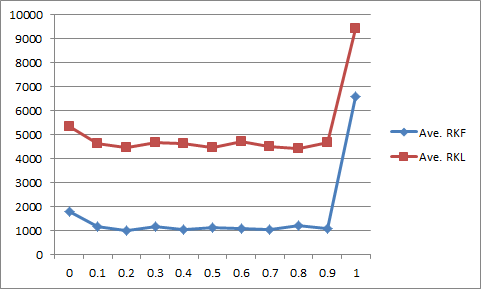
\includegraphics[width=0.4\textwidth]{evalAlpha}
\caption{Behavior of different alpha value in basic random walk}
\label{fig:evalAlpha}
\end{figure}
\textbf{(C) Selection of loss function.}
We need to consider different loss functions on other \\
\textbf{(D) Selection of regularization function.}
We need to test how different regularization methods affect the performance.\\
\textbf{(E) Experiments with different LDA similarity measures.}
\textbf{(F) Experiments on feature selection}
We need to test the effectiveness of some features.
\subsection{Observations and other considerations}
We observe that self-citation also have impact on the performance because the one would likely to cite his own paper if they are on the similar topic. We would like to test our algorithm on a citation network without self-citations.
\subsection{Evaluation result on data set}
We need to present our final results on data set and compare our method with other methods.
\section{Conclusion}

\bibliographystyle{plain}
\bibliography{midrep}
\nocite{*}

\newpage
\section{Appendix}
\subsection{Plan of activities in proposal}
\textbf{Software to write:}\\
We must write feature extractors, modify existing machine learning algorithm implementations
for feature integration and parameter estimation, and create a testing framework.

\textbf{Papers to read:}\\
Ramesh Nallapati, Amr Ahmed, Eric P. Xing, and William W. Cohen, Joint Latent Topic Models
for Text and Citations. Proceedings of The 14th ACM SIGKDD International Conference on
Knowledge Discovery and Data Mining. (KDD 2008)

D. Blei, A. Ng, and M. Jordan. Latent Dirichlet Allocation. Journal of Machine Learning
Research, 3:993–1022, 2003.

\textbf{Midway report milestone:}\\
By this time we will have a system which can rank the citations within a paper, produce a
weighted network, and predict citations using this weighted network. Using this system we can
then evaluate performance by comparing predictions with given citations.

\textbf{Team responsibilities:}\\
Since our task involves a lot of feature engineering we will divide the investigation and
extraction of features equally among our team members. Our remaining tasks include integration
of features into a weight prediction algorithm (Jon), parameter estimation for the weight
prediction algorithm (Kartik), and developing a testing framework for citation predictions
(Zhengzhong).

\subsection{Current plan of activities}
\textbf{Software to write}:\\
We have finish the basic evaluation framework and feature extractors. We still need to merge 
our code of data preparation with our training code. We also need to do more data clean up to get
higher quality features from data. We also need to implement more measures for LDA similarity.

\textbf{Papers to read:}\\
Although we have finished literature review, we still need to read some selected papers in our related works 
again to get a deeper understanding to the problem, important papers including Lao \& Cohen(2010),.Yu et,al (2012) \
and Backstrom \& Leskovec(2011)

\textbf{Future activities:}\\
As the general framework of our project has been established, our future activities will be experiment
centric. We will do experiment on different methods and variations to get the best out from our model. The
most important experiments to do would be feature selection and loss function experiments.

\textbf{Team responsibilities:}\\
Jon will continue work on feature extraction and data clean up, Kartik will work on LDA feature and similarity
measures, and Zhengzhong  will merge project framework and conduct experiments on the model decisions listed in
the Experiment section. All members will help with experiments once the framework is finalized.
\end{document}
